%!TEX root = constraint-layout.tex

% \newcommand{\teaserFigure}{
% 	\teaser{
% 		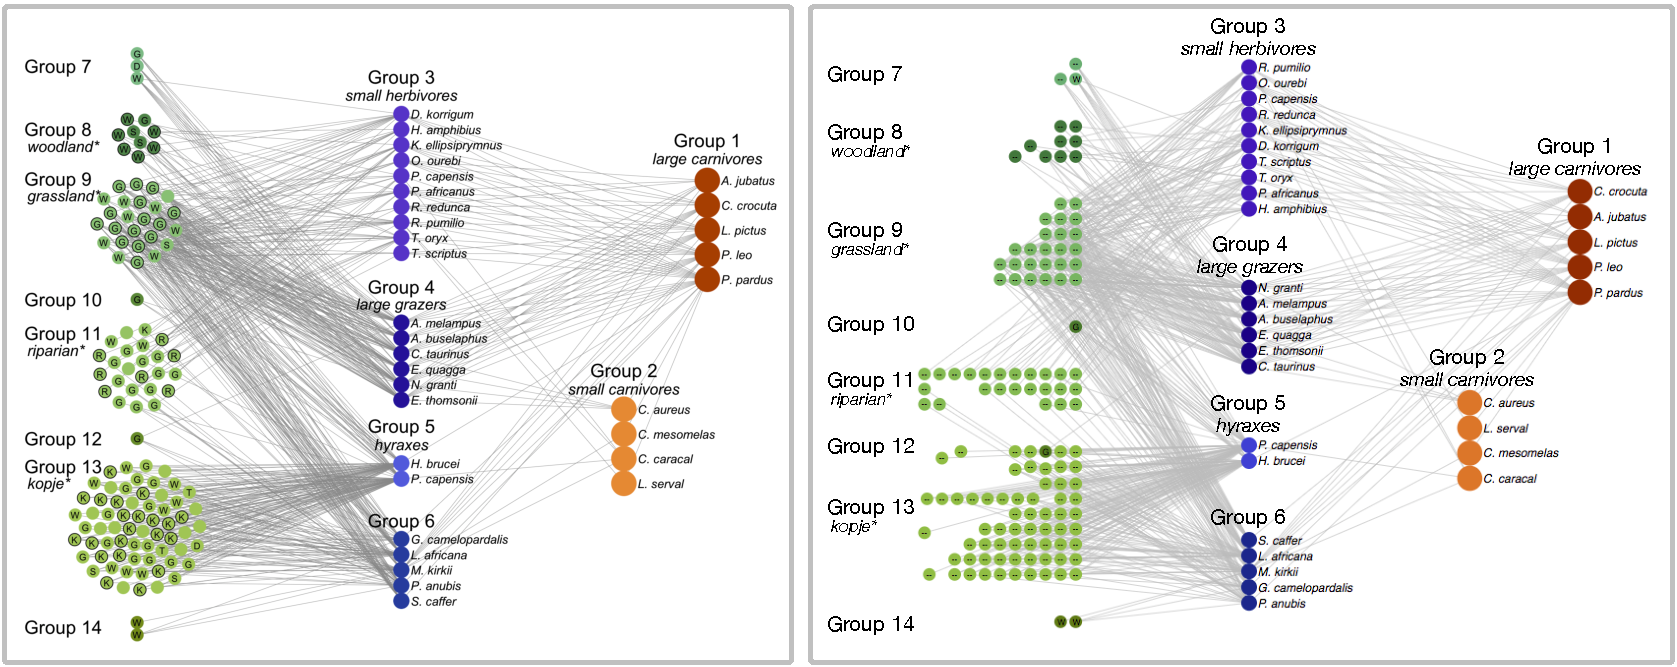
\includegraphics[width=\linewidth]{figures/serengeti-layout.pdf}
% 		\centering
% 	  \caption{\label{fig:teaser}}

% 	}
% }

%%%%%%%%%%%%%%%%%%%%%%%%%%%%%%%%%%
%%%%%%%%%%%%% Design %%%%%%%%%%%%%
%%%%%%%%%%%%%%%%%%%%%%%%%%%%%%%%%%

\newcommand{\smallTreeExample}{
  \begin{figure}[t!]
    \centering
    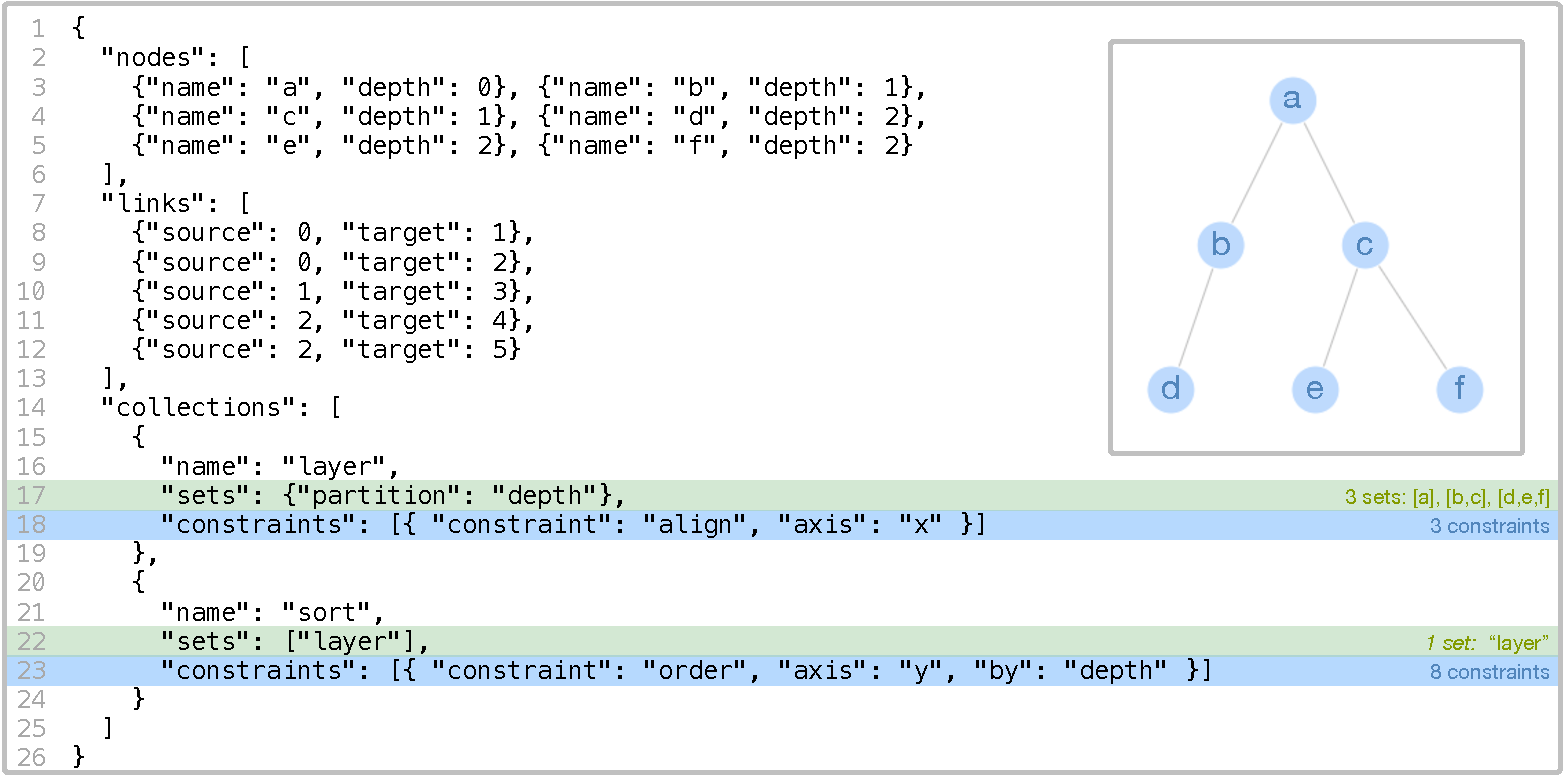
\includegraphics[width=\columnwidth]{figures/small-tree-example.pdf}
      \vspace{-15px} {\caption{\label{fig:small-tree-example} The \projectname specification
      and data for a tree with six nodes. Nodes are split into sets 
      based on their \texttt{depth} and aligned. 
      A new set definition uses composition to include only the ``layer'' set
      and orders each layer by its depth to form the tree.}}
    \vspace{-20px}
  \end{figure}
}

\newcommand{\smallTreeExampleWebCoLa}{
  \begin{figure}[t!]
    \centering
    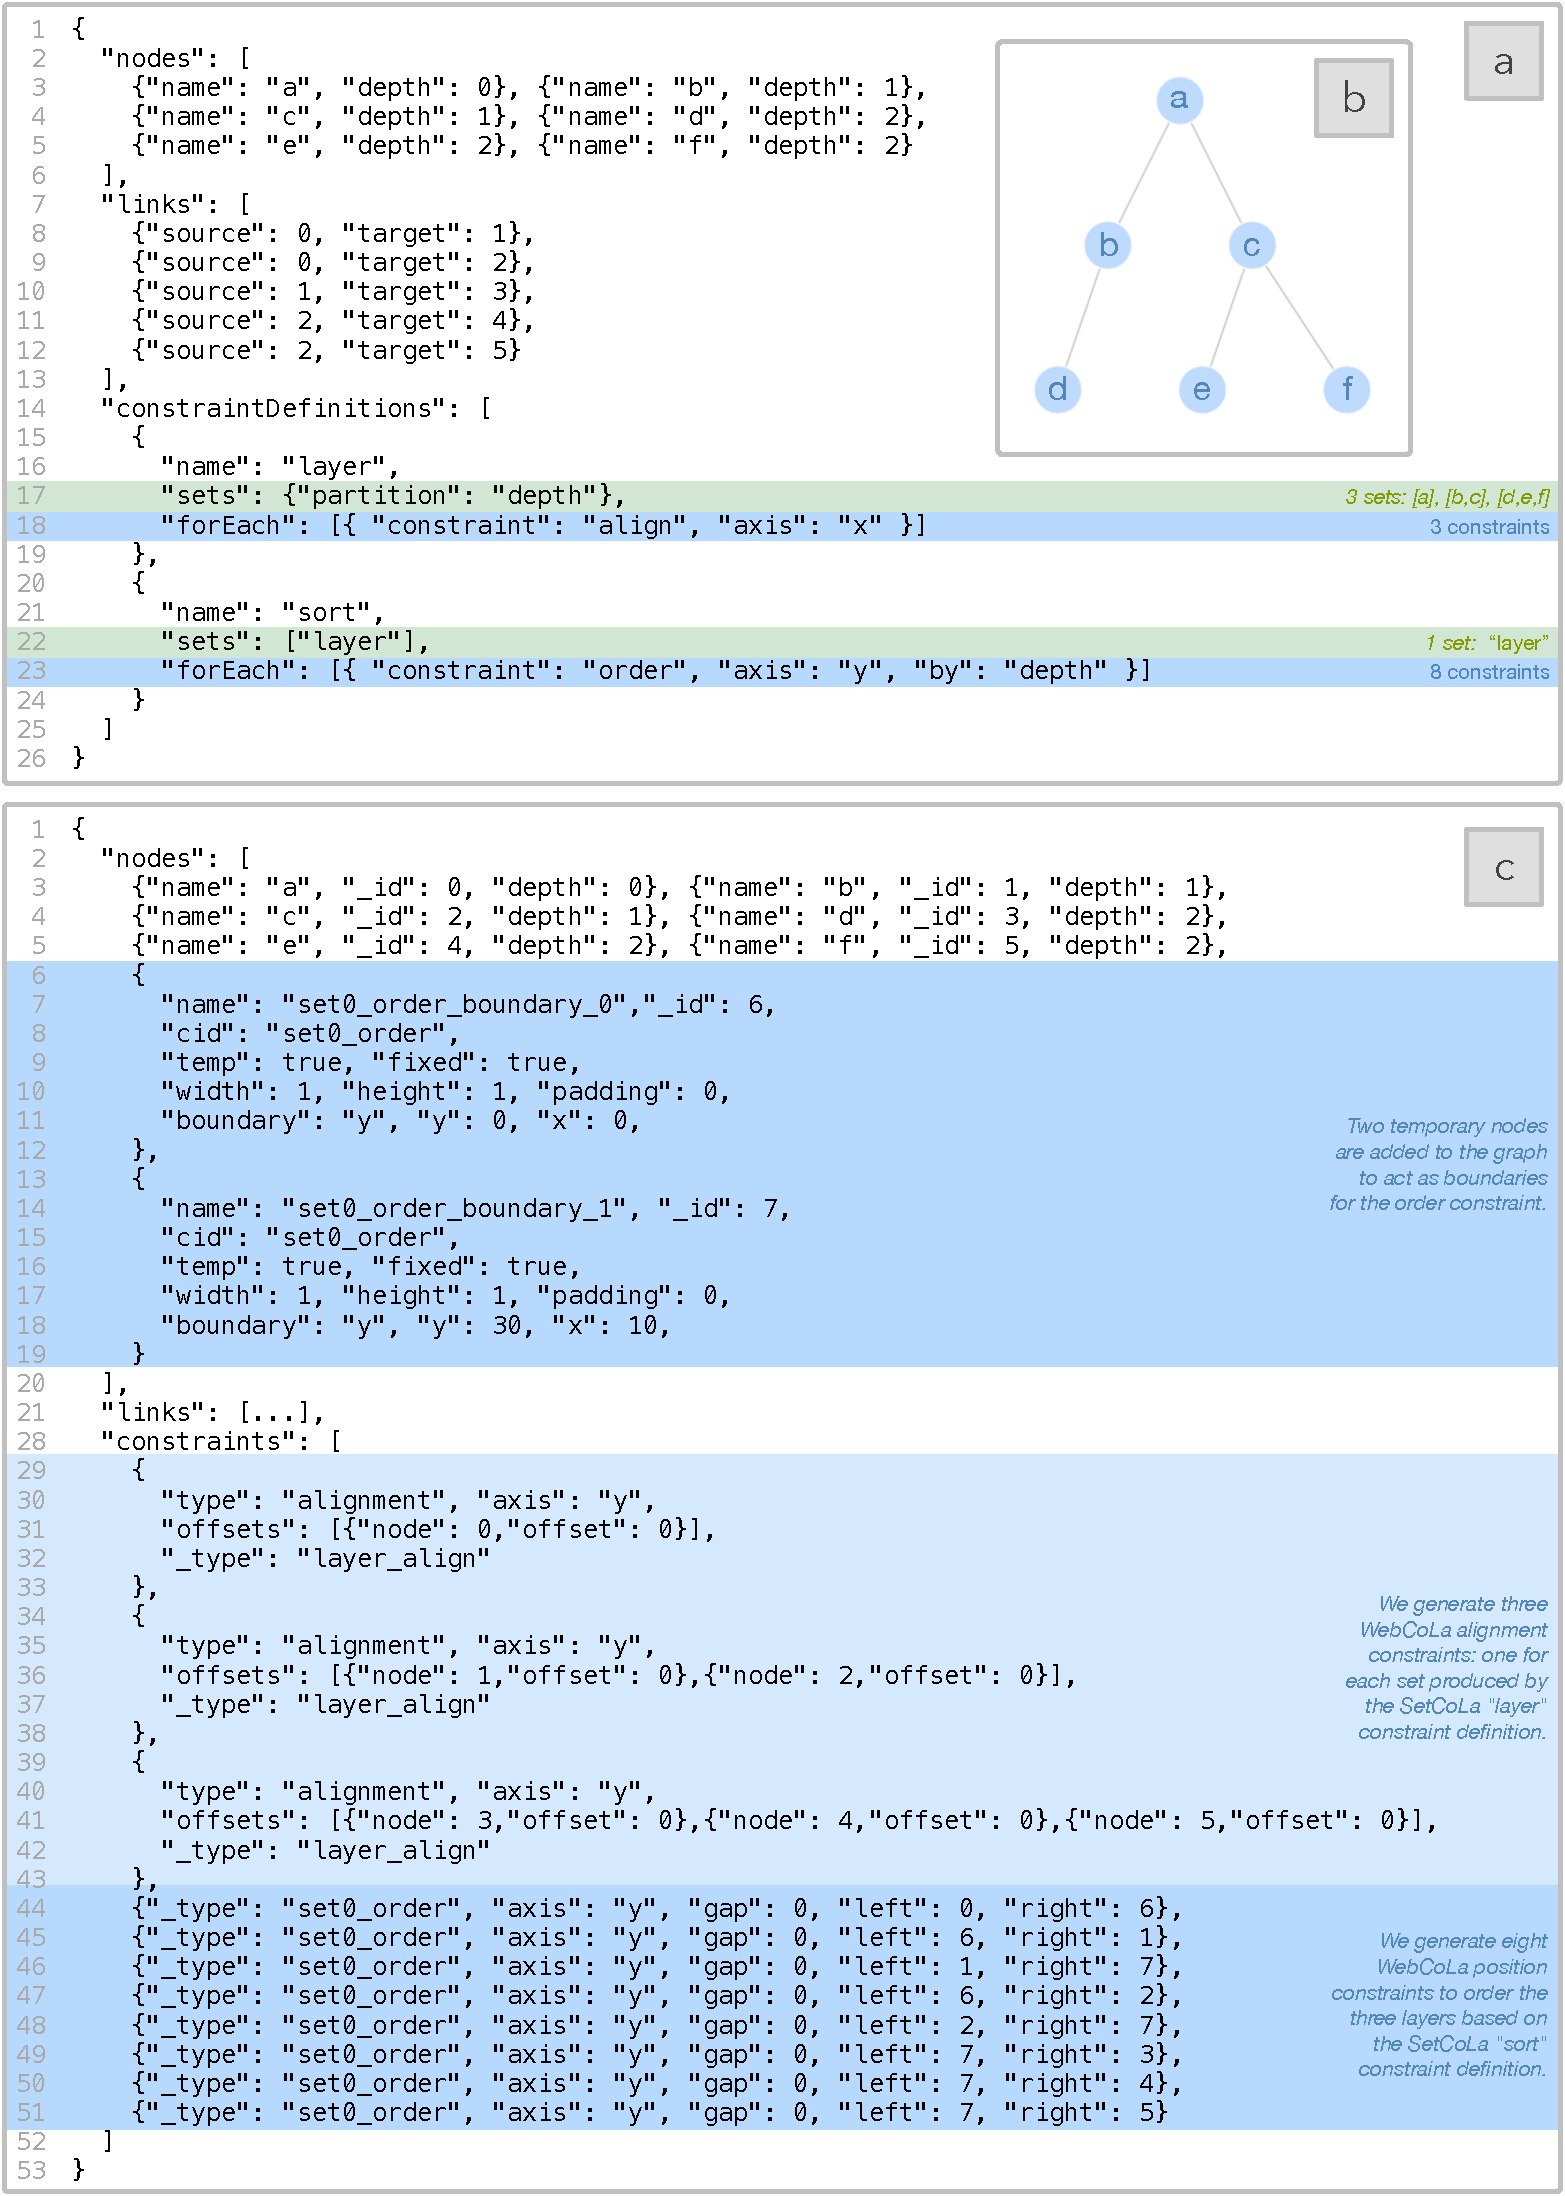
\includegraphics[width=\columnwidth]{figures/small-tree-webcola.pdf}
      \vspace{-15px} {\caption{\label{fig:small-tree-example} 
      (a)~The \projectname specification and data for (b)~a tree with six 
      nodes. Nodes are split into sets based on their \texttt{depth} and 
      aligned. A new set definition uses composition to include only the 
      ``layer'' set and orders each layer by its depth to form the tree.
      (c)~The WebCoLa specification created by the \projectname compiler.}}
    \vspace{-20px}
  \end{figure}
}

%%%%%%%%%%%%%%%%%%%%%%%%%%%%%%%%%%
%%%%%%%%% Demonstration %%%%%%%%%%
%%%%%%%%%%%%%%%%%%%%%%%%%%%%%%%%%%

\newcommand{\krugerLayout}{
  \begin{figure}[t!]
    \centering
    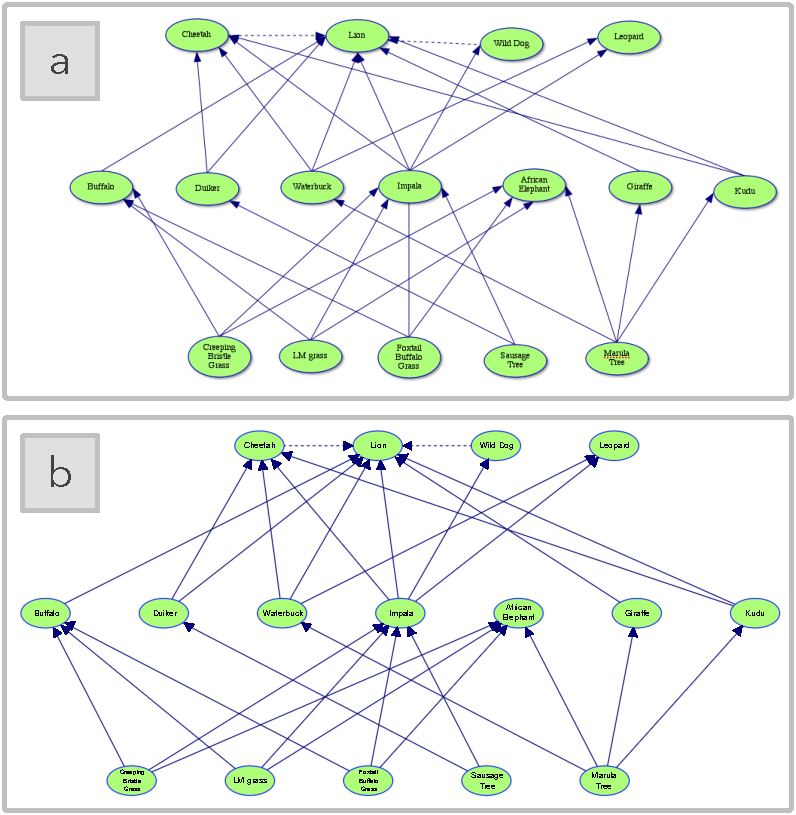
\includegraphics[width=\columnwidth]{figures/kruger-layout.pdf}
    \vspace{-15px} {\caption{
      \label{fig:kruger-layout} A subset of the food web for Kruger 
      National park arranged by trophic level (i.e., carnivore, 
      herbivore, and plant), as seen on the website \cite{kruger2017} 
      and (b) recreated using \projectname.
    }}
    \vspace{-20px}
  \end{figure}
}

\newcommand{\serengetiLayout}{
  \begin{figure*}[t]
    \centering
    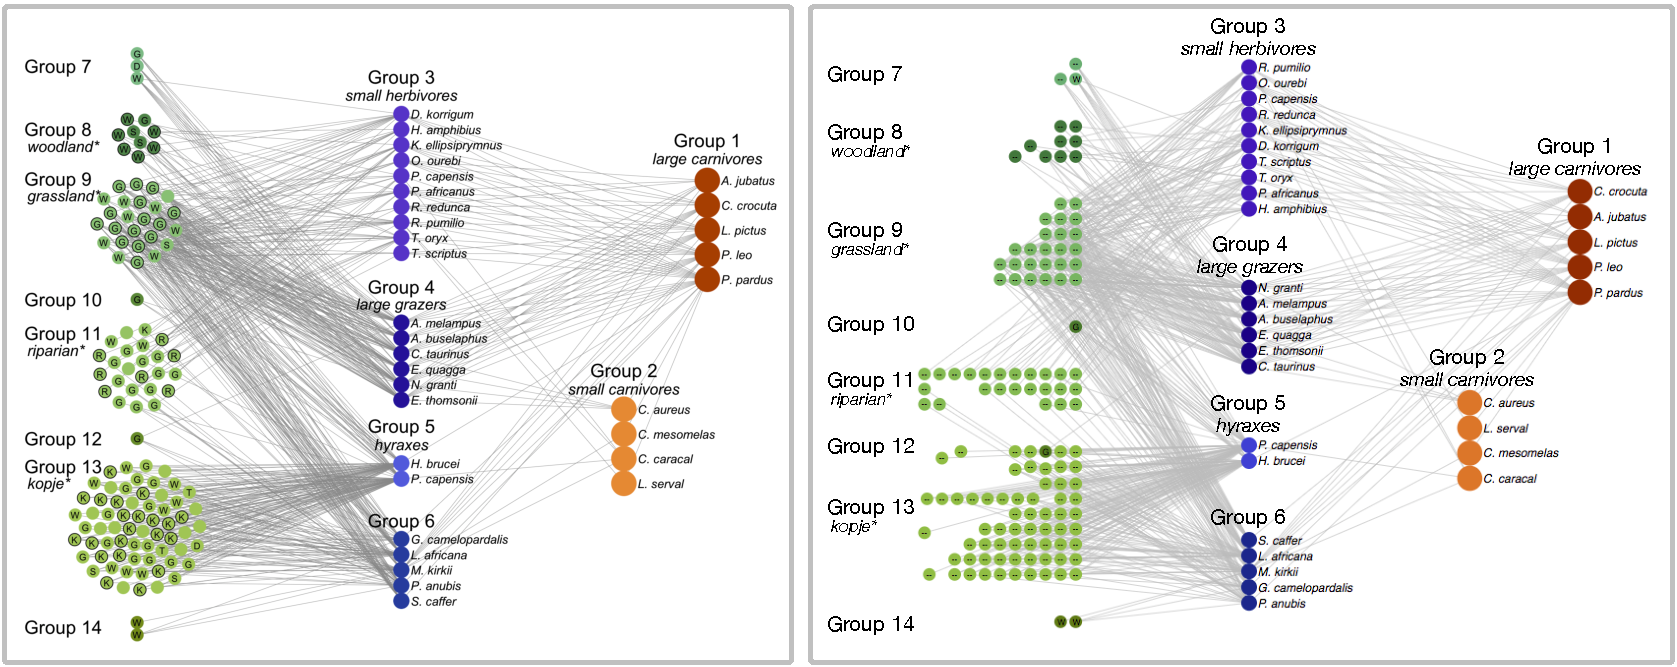
\includegraphics[width=\textwidth]{figures/serengeti-layout.pdf}
    \vspace{-15px} {\caption{\label{fig:serengeti-layout} The layout for
        the Serengeti food web from (a) Baskerville et al.~\cite{baskerville2011spatial}
        as compared to (b) the layout recreated with \projectname.
        Nodes are grouped by trophic level clusters produced from a Bayesian
        analysis method.}}
  \end{figure*}
}

\newcommand{\serengetiSpec}{
  \begin{figure}[h!]
    \centering
    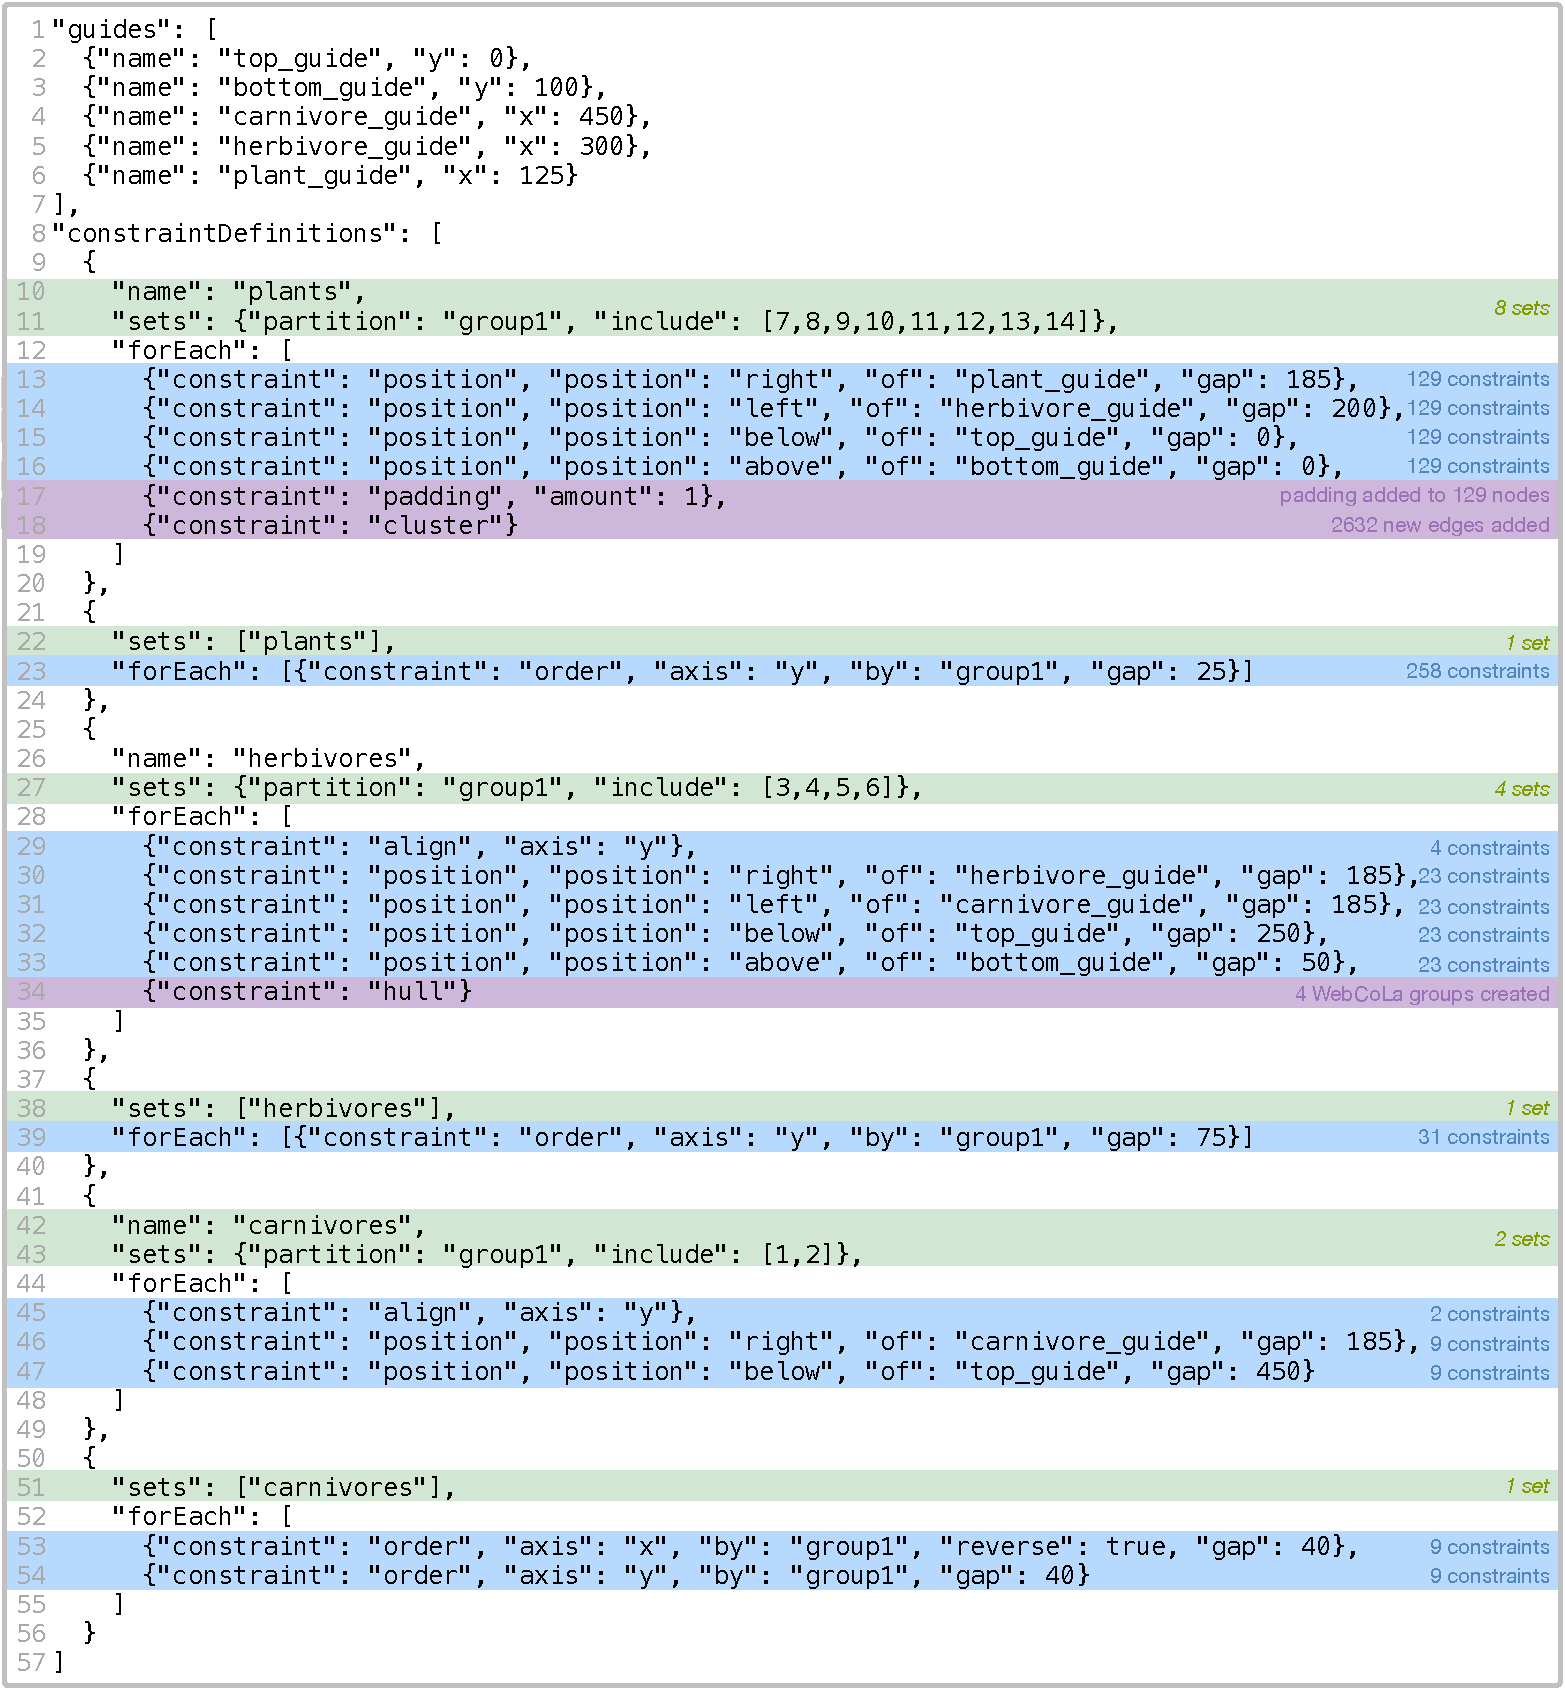
\includegraphics[width=\columnwidth]{figures/serengeti-spec.pdf}
    \vspace{-15px} {\caption{\label{fig:serengeti-spec} The
        \projectname~specification for the Serengeti food web shown in
        Figure~\ref{fig:serengeti-layout}.}}
    \vspace{-10px}
  \end{figure}
}

\newcommand{\syphilisLayout}{
  \begin{figure*}[t]
    \centering
    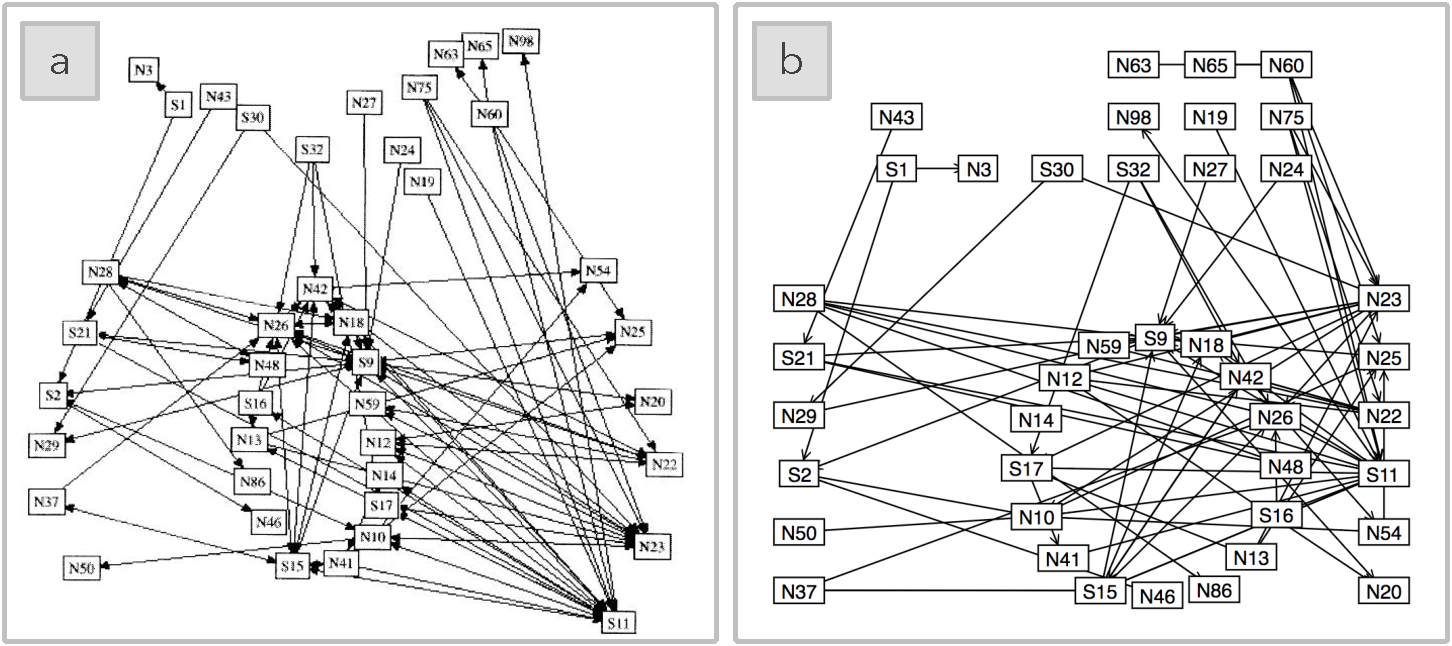
\includegraphics[width=\textwidth]{figures/syphilis-layout.pdf}
    \vspace{-15px} {\caption{\label{fig:syphilis-layout} The layout for the
        syphilis social network from (a) Rothenberg et
        al.~\cite{rothenberg1998using}. (b) We recreated and improved the
        layout in \projectname by introducing additional padding, alignment,
        and circle constraints to further highlight the relative
        number of interactions
        among the different groups. For both figures, the nodes are split
        into three groups, from left to right: young affluent
        white men, younger white women, and young African-American men. Individuals
        not associated with any of these ``core'' groups are positioned above 
        the others.}}
  \end{figure*}
}

\newcommand{\syphilisSpec}{
  \begin{figure}[t]
    \centering
    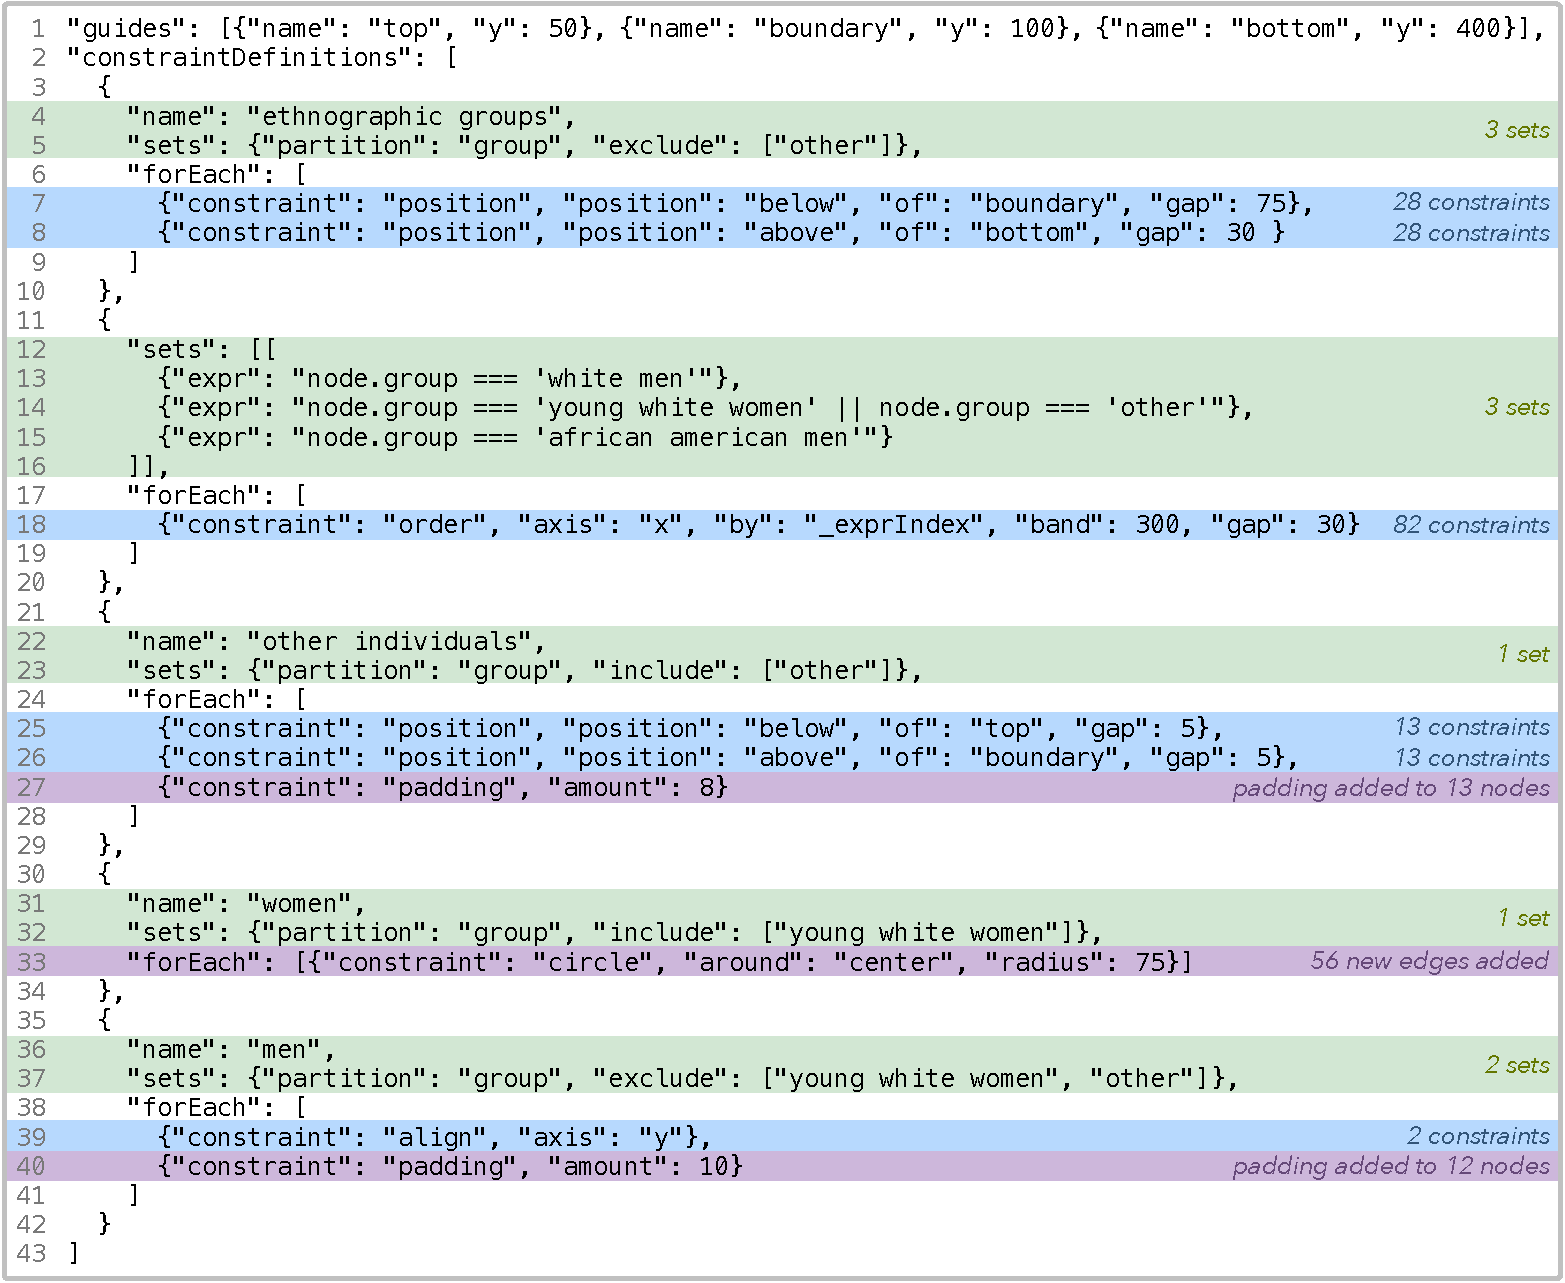
\includegraphics[width=\columnwidth]{figures/syphilis-spec.pdf}
    \vspace{-15px} {\caption{\label{fig:syphilis-spec} The
        \projectname~specification for the syphilis social network shown in
        Figure~\ref{fig:syphilis-layout}. The code is annotated with the
        number of sets produced (green), the number of WebCoLa constraints
        generated for the final layout (blue), and the behavior of \projectname
        constraints \emph{not} converted to WebCoLa (purple).
    }}
  \end{figure}
}

\newcommand{\tlrfourLayout}{
  \begin{figure}[t!]
    \centering
    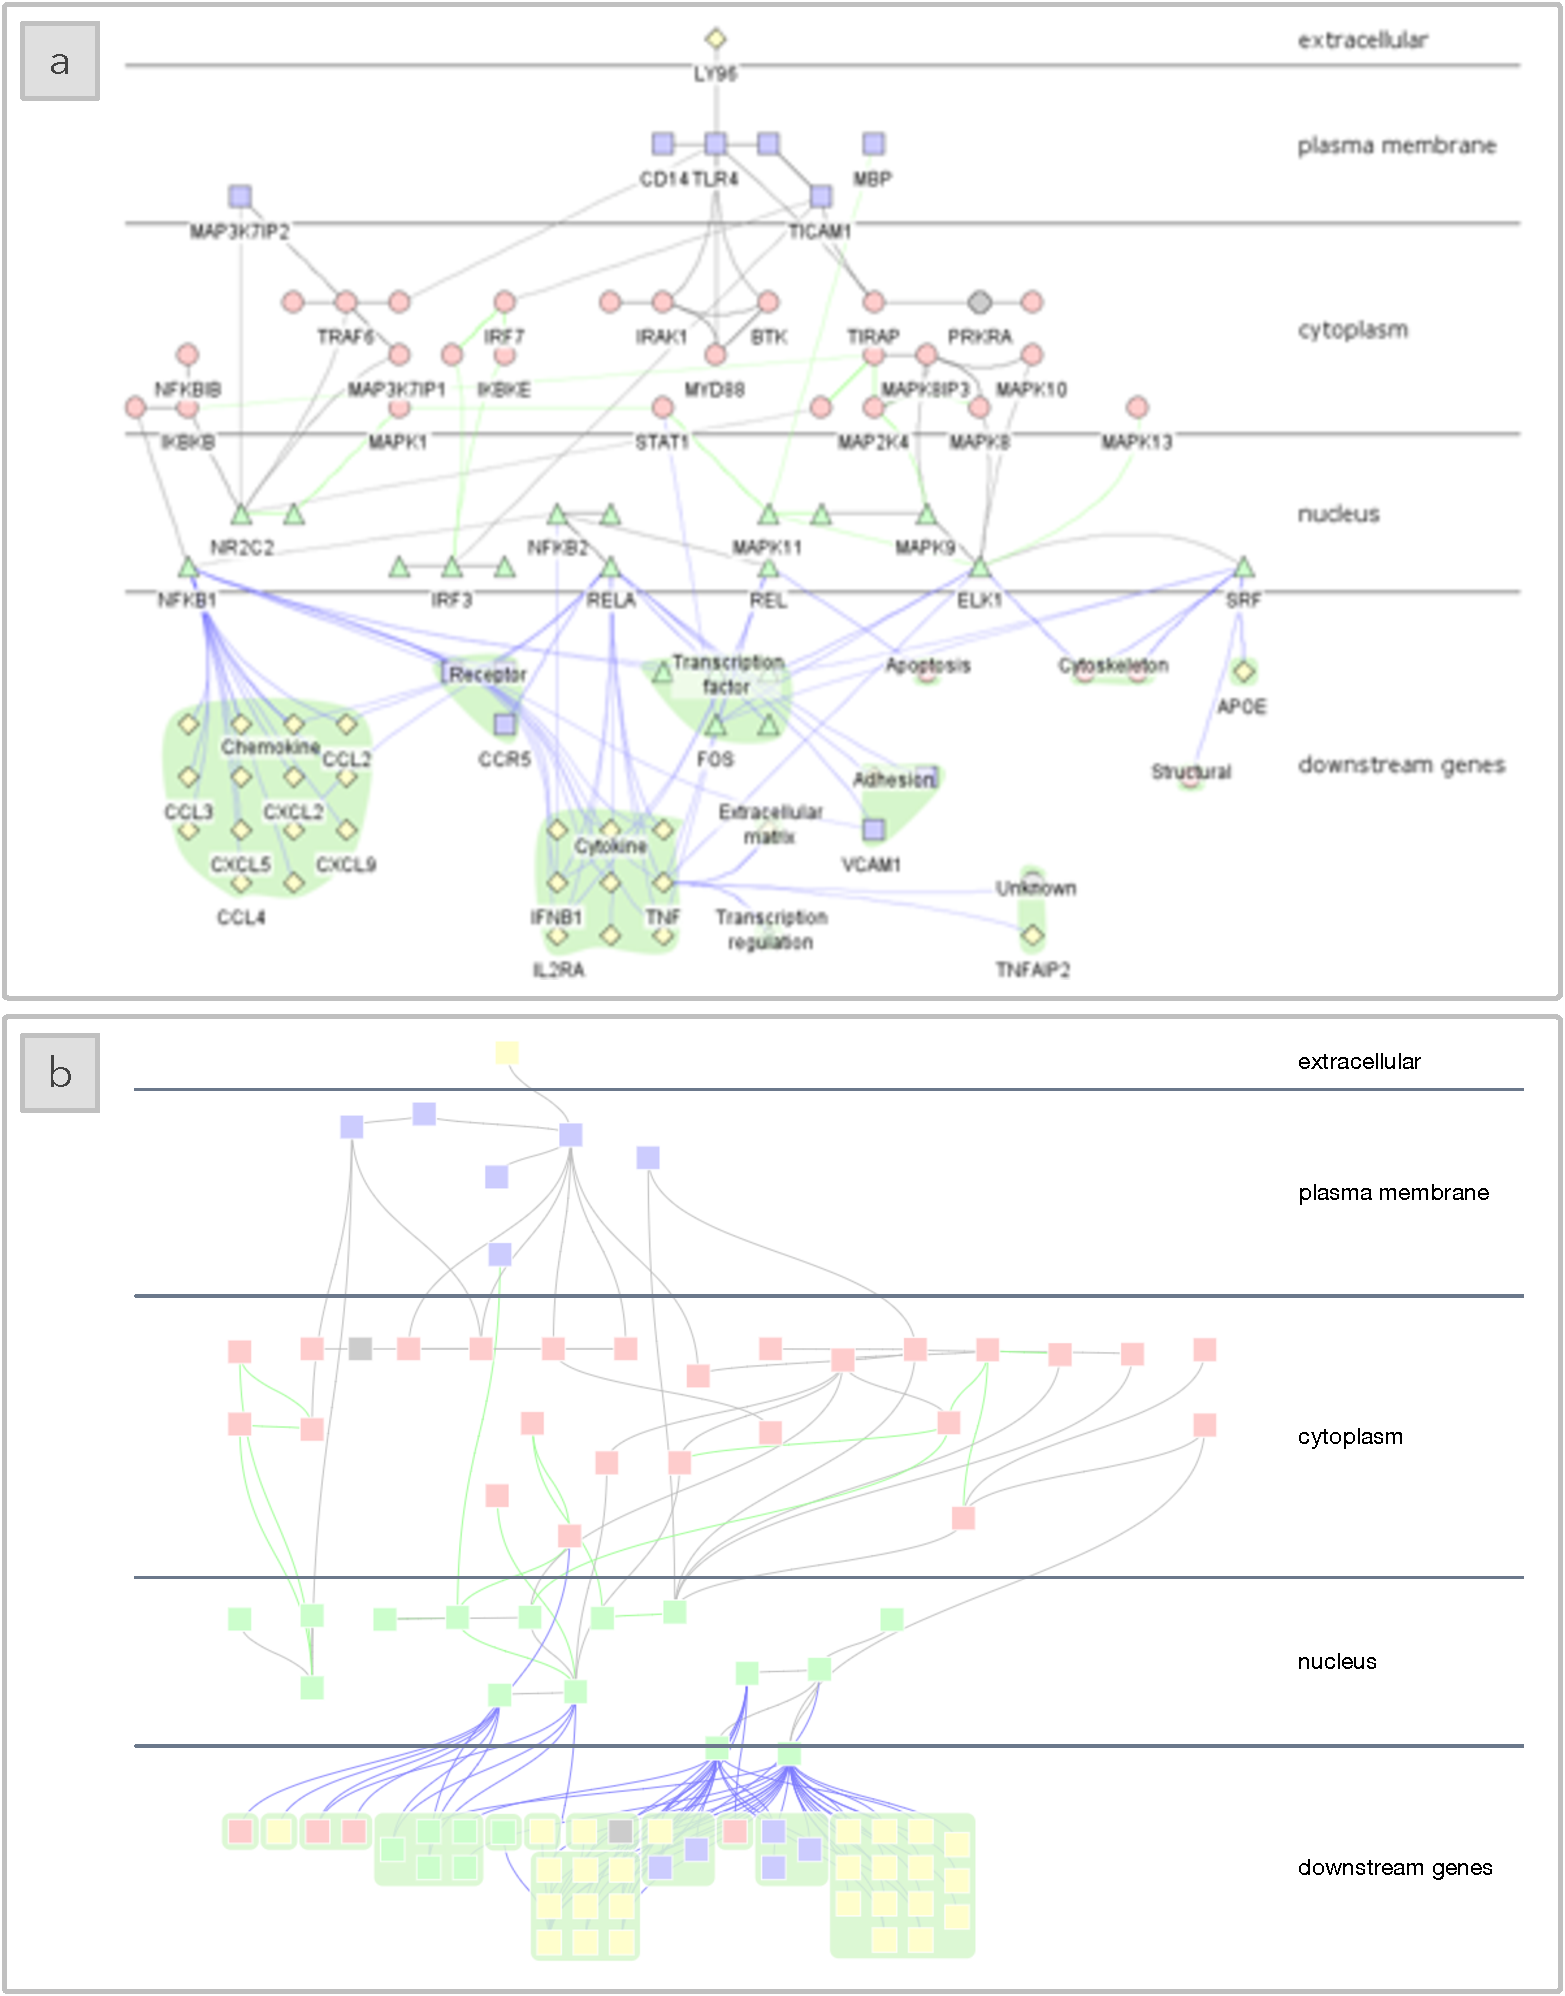
\includegraphics[width=\columnwidth]{figures/tlr4-layout.pdf}
    \vspace{-11px} {\caption{\label{fig:tlr4-layout} The layout for
        the TLR4 biological system produced using (a) Cerebral~\cite{barsky2008cerebral},
        a domain-specific layout tool, as compared to (b) \projectname.
        The layers correspond to the location of the biomolecule 
        within a cell and show immune response outcomes at the bottom of
        the graph, grouped by molecular function.
    }}
    \vspace{-40px}
  \end{figure}
}

\newcommand{\tlrfourSpec}{
  \begin{figure}[t]
    \centering
    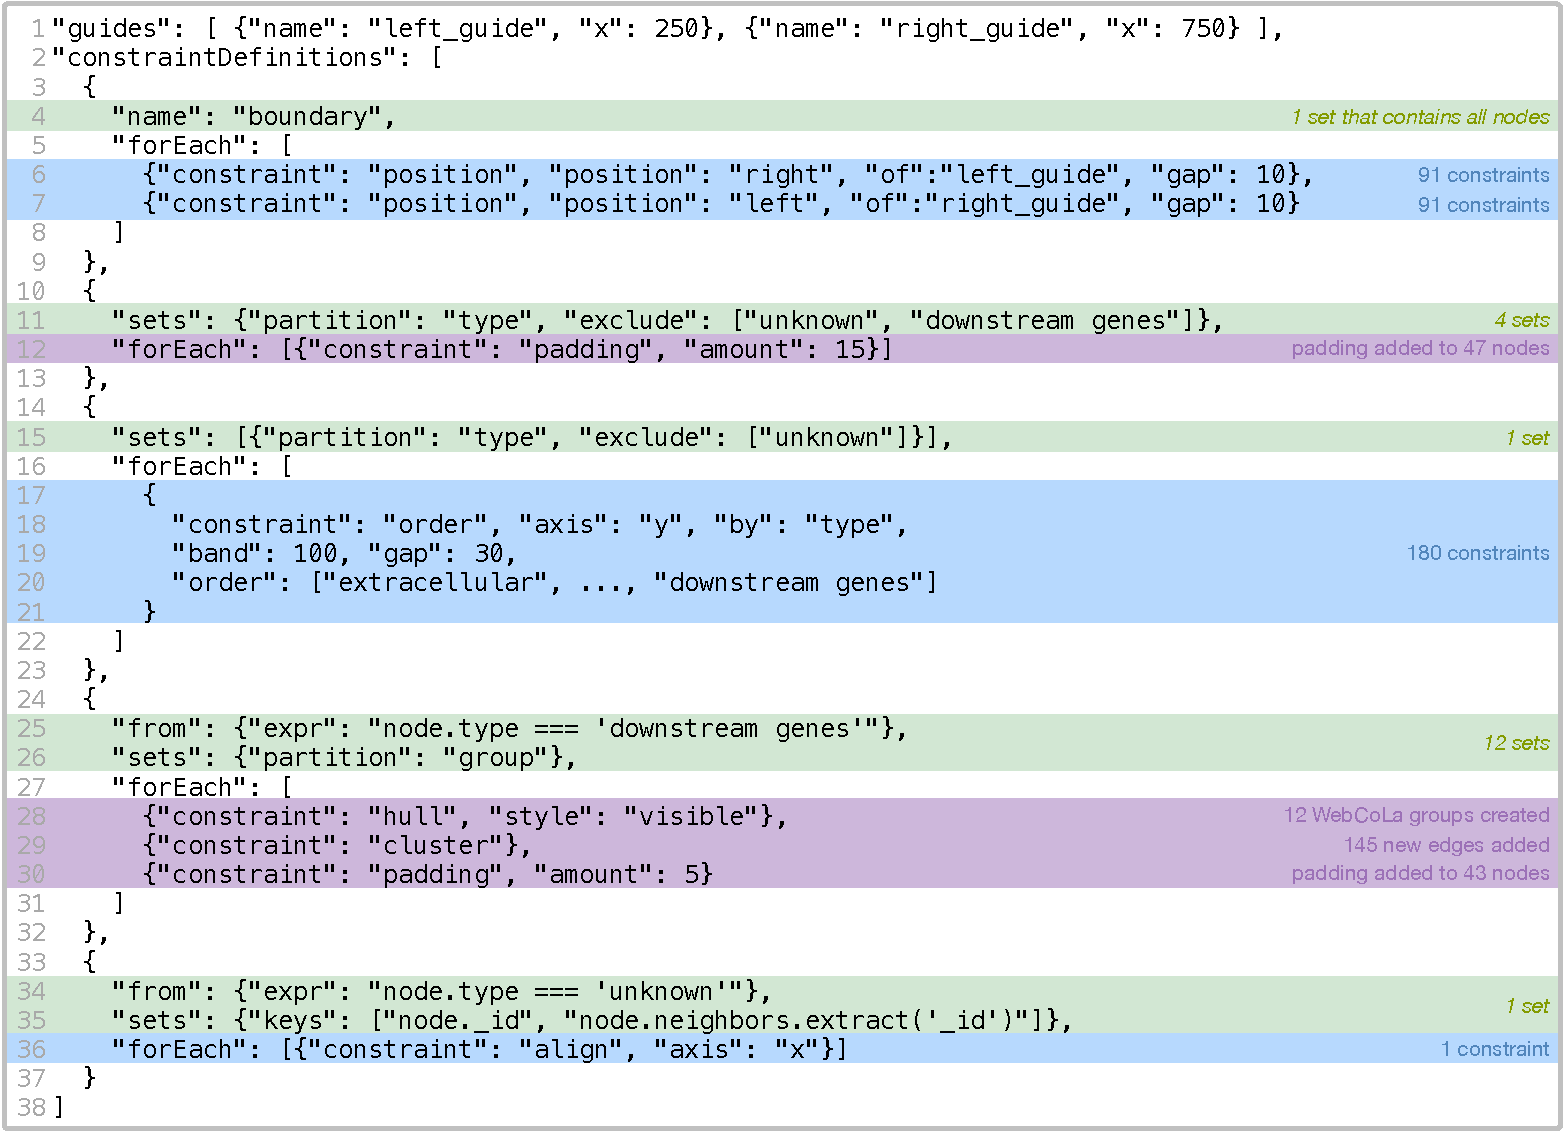
\includegraphics[width=\columnwidth]{figures/tlr4-spec.pdf}
    \vspace{-15px} {\caption{\label{fig:tlr4-spec} The
        \projectname~specification for the TLR4 biological system shown in
        Figure~\ref{fig:tlr4-layout}.}}
  \end{figure}
}

\newcommand{\constraintsFigure}{
  \begin{figure*}[t]
    \centering
    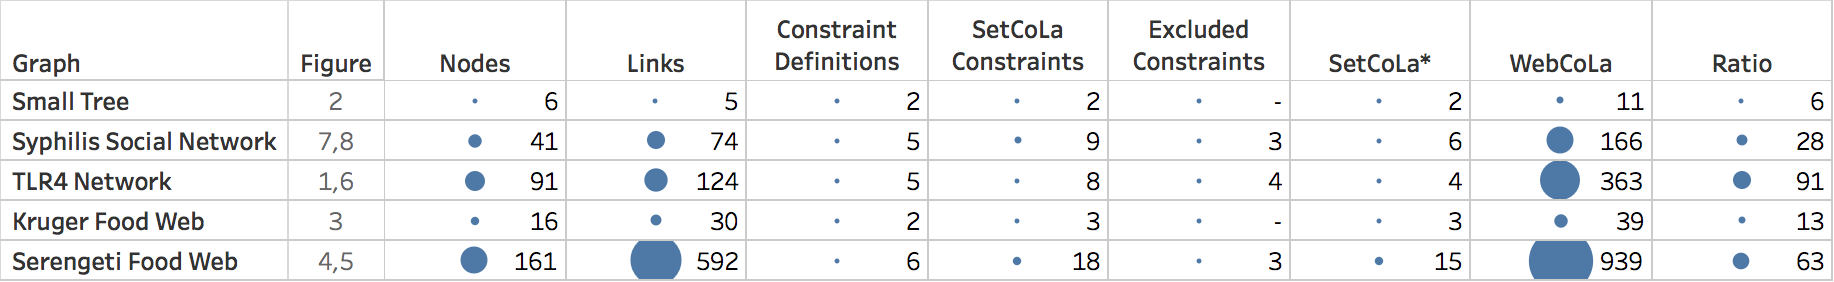
\includegraphics[width=\textwidth]{figures/constraints.png}
    \vspace{-15px} {\caption{\label{fig:constraints} The number of nodes,
        links, and constraints for each example.  The columns labeled
        \textbf{Constraint Definitions} and \textbf{\projectname Constraints}
        list the number of these definitions or constraints
        written by the user.  Since some \projectname constraints are not
        directly converted to WebCoLa, we also tabulate the number of such
        constraints (\textbf{Excluded \projectname Constraints}) and compare the reduced
        number (\textbf{Comparable \projectname Constraints}) to the 
        number of \textbf{WebCoLa Constraints} generated by the \projectname compiler,
        to determine the increase factor (\textbf{Ratio}).}}
  \end{figure*}
}
